
        \begin{abstract}{Bridging Scales for Simulation of Lipids}{%
            S. Roy}{%
            Prescience Insilico Pvt. Lmtd.}{%
            \IStag}
        The design of supramolecular nanostructures for drug delivery is hindered by a limited atomistic level understanding of interactions between building blocks. Here, we report the development of a computational algorithms integrates force-field-based models with large-scale all-atomistic explicit water molecular dynamics simulations to mesoscale simulation to design stable nanoscale lipidic supramolecular structures. In one example, we demonstrate how optimizing the ratio of excipients can help in forming stable nanoscale supramolecular assembly with different phases. In our second example we showcase the self-assembly of sophorolipids which contained hydrophilic head groups at the ends of a long hydrophobic tail. As a result of dual head groups sophorolipids can self assemble into variety of structures (morphologies) in water. Distinctions in structural arrangements of these self assembled systems along with the phase diagram as a function of concentration in water from mesoscale simulations will be presented. \begin{center}  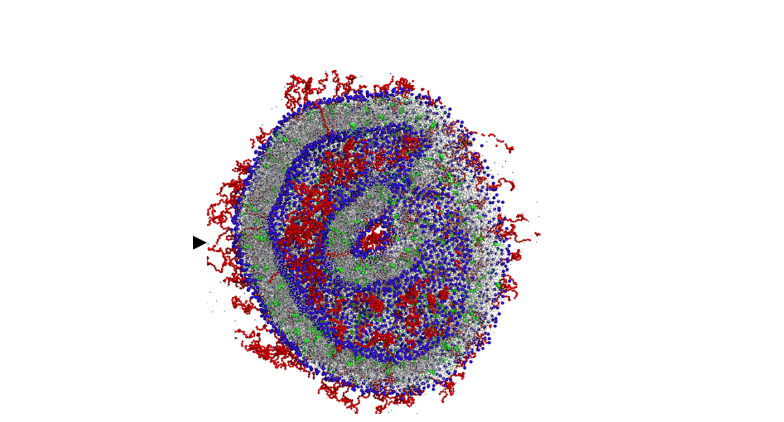
\includegraphics[width=\linewidth]{abstracts/txt/figures/sudip.png}  \caption{Self-assembled supramolecule for drug delivery.}  \end{center}  
        \end{abstract}
        